\section{Components}
\label{sec:components}
Just like in Unity, the components are the building blocks of the game objects.
They are the individual features that can be added to a game object to give it functionality.

\subsection{class diagram}
\begin{figure}[H]
    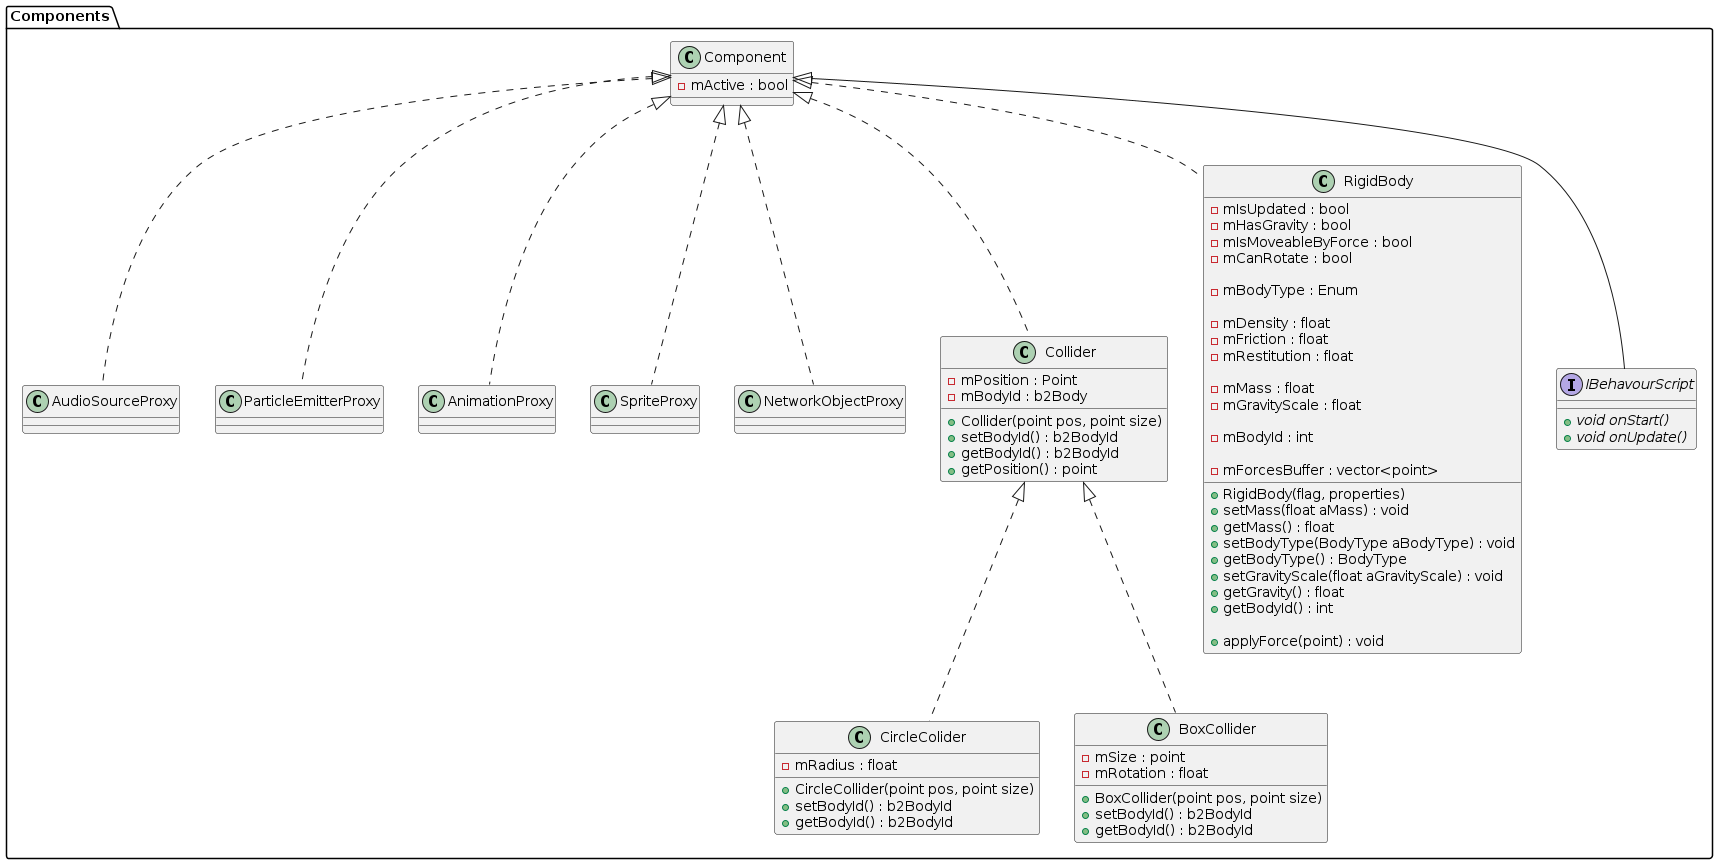
\includegraphics[width=1.2\textwidth]{componentsPackageClassDiagram.png}
    \caption{Class diagram of the components. Note that the components here are called proxies, because they do not contain the actual members of the component. See the full diagram for their complete functionality.}
    \label{fig:components}
\end{figure}

\subsection{AudioSource}
See \autoref{sec:audio} for more information.
Used to add audio to a GameObject.

\subsection{Collider}
Has \texttt{bodyID}, which is needed for the physics.

\subsection{NetworkObject}
see \autoref{sec:networking} for more information.

\subsection{Sprite}
Used to add a still image to a GameObject.
See \autoref{sec:rendersystem} for more information.

\subsection{Animation}
Used to add an animated image to a GameObject.
See \autoref{sec:rendersystem} for more information.

\subsection{Collider}

\subsection{CircleCollider}

\subsection{BoxCollider}

\subsection{RigidBody}
Has \texttt{bodyID}, which is needed for the physics.

\subsection{IBehaviourScript}
IBehaviour script is an interface that can be used to create behaviour scripts for GameObjects.

\subsection{ParticleEmitter}
Particle emitter is a component that can be used to create particle effects.
See \autoref{sec:particlesystem} for more information.

\subsection{AudioSource}
Used to add audio to a GameObject. See chapter \autoref{sec:audio} for details

\subsection{Transform}
The Transfrom is not a class but a struct. It represents the position, rotation and scale of a GameObject.
Does not need an update flag when the position is changed, as a movable object is usually moving.


